\documentclass[letterpaper,twocolumn,fleqn]{article} 

\pagestyle{empty}                % no page numbers is default

\usepackage{amsfonts}
\usepackage{amssymb}
\usepackage[cmex10]{amsmath}
\usepackage{booktabs}
\usepackage{caption}
\usepackage{enumitem}
\usepackage{graphicx}
\usepackage{fancyvrb}
\usepackage{framed}
\usepackage{ifthen}
\usepackage{cite}
\usepackage{tabulary}
\usepackage{url}
\usepackage{xspace}
\usepackage{wrapfig}
\usepackage[pdfborder={0 0 0}]{hyperref}
\usepackage{verbatim}

\usepackage{ist} % Style for IST in package instead of document class.

\usepackage{color}
\definecolor{yellow}{rgb}{1,1,0}
\definecolor{black}{rgb}{0,0,0}
\definecolor{ltcyan}{rgb}{.75,1,1}
\definecolor{red}{rgb}{1,0,0}
\definecolor{gray}{rgb}{.6,.6,.6}
\definecolor{darkred}{rgb}{0.5,0,0}
\definecolor{darkgreen}{rgb}{0,0.5,0}

% Cite commands I use to abstract away the different ways to reference an
% entry in the bibliography (superscripts, numbers, dates, or author
% abbreviations).  \scite is a short cite that is used immediately after
% when the authors are mentioned.  \lcite is a full citation that is used
% anywhere.  Both should be used right next to the text being cited without
% any spacing. \hcite is a citation that I am hiding, perhaps because I am
% nearing the maximum number of citations for a journal.
\newcommand*{\lcite}[1]{~\cite{#1}}
\newcommand*{\scite}[1]{~\cite{#1}}
\newcommand*{\hcite}[1]{}

\newcommand{\etal}{et al.\xspace}

\newcommand*{\keyterm}[1]{\emph{#1}}

\newcommand{\fix}[1]{{\color{red}\textsc{[#1]}}}
%\newcommand{\fix}[1]{}

% Avoid putting figures on their own page.
\renewcommand{\textfraction}{0.05}
\renewcommand{\topfraction}{0.95}
\renewcommand{\bottomfraction}{0.95}

% Make sure this is big enough so that only big figures end up on their own
% page but small enough so that if a figure does have to be on its own
% page, it won't push everything to the bottom because it's not big enough
% to have its own page.
\renewcommand{\floatpagefraction}{.75}


\title{Why We Use Bad Color Maps and What You Can Do About It}

\author{Kenneth Moreland; Sandia National Laboratories; Albuquerque, New
  Mexico, USA}

\date{} % date has an empty field.

% correct for bad hyphenation here
\hyphenation{Para-View}

\begin{document} 

\maketitle 

\thispagestyle{empty} % prevents the first page to be numbered

\begin{abstract}
\noindent
We know the rainbow color map is terrible and emphatically reviled by the
visualization community, yet its use continues to persist. Why do we
continue to use a this perceptual encoding with so many known flaws?
Instead of focusing on why we should not use rainbow colors, this position
statement explores the rational for why we do pick these colors despite
their flaws. Often the decision is influenced by a lack of knowledge, but
even experts that know better sometimes choose poorly. A larger issue is
the expedience that we have inadvertently made the rainbow color map
become. Knowing why the rainbow color map is used will help us move away
from it. Education is good, but clearly not sufficient. We gain traction by
making sensible color alternatives the more convenient alternative. It is
not feasible to force a color map on users. Our goal is to supplant the
rainbow color map as a common standard, and we will find that even those
wedded to it will migrate away.
\end{abstract}


\section{Introduction}

\noindent
A pervasive technique in scientific visualization called pseudocoloring is
to apply colors to an object that vary based on some numerical variable.
Pseudocoloring requires defining a function or map from numerical values to
colors. A color map is typically defined by selecting a continuum of colors
that map linearly to a range of numeric values.
Figure~\ref{fig:ColorMapExample} shows a simple example of a color map
where numeric values between -1 and 0 map to blue colors of varying
brightness and numeric values between 0 and 1 map to red colors.

\begin{figure}[htb]
  \centering
  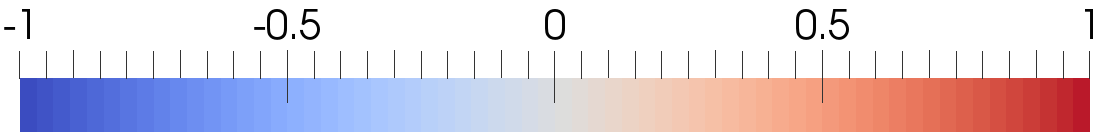
\includegraphics[width=.9\linewidth]{images/ColorMapExample}
  \caption{A simple example of a color map.}
  \label{fig:ColorMapExample}
\end{figure}

The efficacy of a pseudocolor visualization is contingent on the ability of
a human observer to translate the colors back into the numeric values they
represent. The choice of colors used in a pseudocolor map can have a major
impact on this inverse translation. Consequently, much research has focused
on the perception of color and its impact of the visual display of
data\fix{cite stone, brewer, ware, reigens, rogowitz}. As one might expect,
the color choice can have a dramatic impact on a viewer's performance in
interpreting colors as numbers, and many effective color sets have been
designed for this purpose.

With this rich understanding of color perception, one might think that
modern visualizations make effective use of color. Unfortunately, many
visualizations today use color sets that are known to be extremely
problematic. In particular the rainbow color map, so called for its use of
the spectrum of colors in the rainbow, is pervasively used in visualization
despite the copious evidence that it performs poorly\fix{cite Borland,
  Reigens, Franchesca? Others?}.

This paper is a retrospective on why these bad colors are so commonly
chosen for visualization and is a position statement on what we as
practitioners can do to best promote good color use.

\fix{I am considering having a short section on the evils of the rainbow
  color map if there is room. If I do, I might remove a few lines above. If
  I do not, I might add a statement or two above that we are not addressing
  this because it is so commonly presented.}


\section{Why We Use Bad Colors}

\noindent
Reserach shows that subjects tend to overestimate their ability to
interpret rainbow colors\fix{cite}. That is, users think they are
interpreting rainbow colors better than alternatives even though they are
in fact doing worse. This is certainly a contributing factor to the
proliferation of the rainbow color map, but not the entire reason. Why else
would the rainbow color map be so profuse in publications by the
visualization community itself, a community that should know
better\fix{cite Borland}?

\subsection{Simplicity}

\noindent
One explanation is the sheer simplicity of creating the rainbow color map.
Nearly all color selections in computer graphics interfaces are done with
RGB (red-green-blue) channels. RGB is a natural choice in computer graphics
because the triplet values match the intensity of red, green, and blue
light mixed in most display peripherals. An unintended consiquence of the
RGB color space is that one of the easiest color continua to make is an
interpolation between different combinations of fully active and fully
inactive channels, which are in fact the rainbow colors. Many computer
graphics interfaces also allow colors chosen with HSV
(hue-saturation-value) channels. The HSV color space makes makes rainbow
colors even easier: hold saturation and value at maximum while varying hue.

With the simplicity of creating a rainbow spectrum of colors combined with
the inclination to accept the colors as a good representation, it is no
wonder that the rainbow colors are often the first and likely the default
color mapping introduces as a visualization package gets built. These
initial poor color choices quickly become ingrained in the software as
regression testing and backward compatibility must be maintained. Further
software layers continue to accept this default and software applications
are likely to expose the rainbow color map as its default choice for end
users. Few users will have either the knowledge or the inclination to
change the default colors used, and thus the rainbow color map becomes
featured throughout visualizations.

\subsection{Aesthetics}

\noindent
However, simplicity is not the only reason rainbow colors are so widely
used. If that were the case, simply making a better alternative would
eradicate the use of bad colors. But this, at least anecdotally, is shown
not to be the case. Consider, for example, bug number 7024 for the ParaView
scientific visualization
application.\footnote{\url{http://www.paraview.org/Bug/view.php?id=7024}} A
user raised this bug soon after the default color map in ParaView was
changed from the rainbow color map to the map shown in
Figure~\ref{fig:ColorMapExample}, which is designed to be reasonably
similar to the rainbow color map it supplants but with better perceptual
characteristics\fix{cite my paper, perceptual studies on it}. Despite this
movement to make the better color map easier, this bug report is an
artifact of the user's difficulty as he went through the extra motions to
go back to the rainbow color map.

The overestimation of the efficacy of the rainbow color map might be a
motivator to spend effort to go back to it, but it is unlikely to be a very
strong motivator. In fact, other ancdotal incidents suggest that even users
that are aware of the rainbow's flaws still have an affinity to use it.
Consider the example visualization in Figure~\ref{fig:ExpertRainbowVis}
created by one of my colleagues at Sandia National Laboratories. He and I
have had many spirited conversations about color use and still he finds
occasion to use the rainbow's colors. His argument is that this particular
visualization is not used for scientific study but rather for communicating
and engaging with non-experts, and these eye-grabbing colors are the best
for this purpose.

\begin{figure}[htb]
  \centering
  \fix{Example frame of bullet hitting apple.}
  \caption{Despite having years of experience and being well aware of the
    problems with rainbow color maps, the designer of this visualization
    chose these colors over others offered with better perceptual
    properties.}
  \label{fig:ExpertRainbowVis}
\end{figure}

Ultimately it is the eye-grabbing nature of the rainbow colors that keeps
us coming back to them over and over again. Regardless of how we can
interpret these colors, the bright and varying pure colors are certainly
captivating (if not distracting), and it takes a good deal of time and
expertise to beat these colors on aesthetics alone.

\subsection{Inertia}

\noindent
Finally, a major contributor to the persistence of the rainbow color map is
that it has become entrenched in scientific visualization. Take for example
VTK\fix{cite}, the popular visualization library. Despite the fact that
better color maps have been used with and contributed to VTK, the default
coloring still reverts to the rainbow map. The problem is that although it
is easy to add a new feature to VTK is easy, changing a core feature like
the default colors is difficult. VTK contains hundreds of regression tests
that could break if the default colors are changed, and updating them can
be very time consuming. Furthermore, such a change will necessarily break
backwards compatibility and so has to be approved by the larger VTK
community, another time consuming process. These software development
minutiae create inertia in changing color map usage.

The same type of inertia forms within scientific communities using
visualization tools. Often scientists compare current results with previous
results. If previous scientific results are only available with the rainbow
color map, the community is stuck with these color choices.


\section{How We Can Promote Good Color Use}

\noindent
Providing and encouraging good color use in visualization is an ongoing
battle. There are many activities the visualization research and
development community can do, and likely all will be required to some
degree.

\subsection{Education}

\noindent
Much research has shown that subjects tend to overestimate the efficacy of
the rainbow color map\fix{cite Borkin2011, others}. Thus, it is critical
that visualization practitioners are educated on the appropriate use of
color.

Fortunately, the visualization community has been vigilant in recent years
to train its own practitioners in good color usage, and there is evidence
that we have made progress. Borland and Taylor\fix{cite} report that 52\%
of papers in the 2005 IEEE Visualization conference proceedings displaying
data with a pseudocoloring use a rainbow color map. In contrast in the
2014 IEEE Visualization conference proceedings, only 29\% (8 out of 28)
papers featuring the pseudocoloring of a 3D scalar field use a rainbow
color map, and only 16\% (10 out of 62) papers feature the color
representation of any sequential data use a rainbow color map. Progress is
being made.

However, education has its limits. Although it might be feasible to educate
visualization practitioners, it is unlikely we can reach every potential
visualization user. Visualization is an integrated part of computational
science, and many tools are designed with the understanding they will be
used by the visualization layman. Furthermore, as we have seen previously
it is often the case that even after having enough education to know the
rainbow color map is bad users still tend to apply it. Education is
necessary, but not sufficient.

\subsection{Admonishment}

\noindent
When education is not quite enough to prevent bad color usage, sometimes a
little push is in order. When we see colors that we know are bad, we should
take the time to attempt getting the creator to fix them. Sometimes this is
simply informing the person. Sometimes it involves some admonishment.

Apart from face-to-face meetings with colleagues, there are many
opportunities to redirect visualizations that go astray. One of the best
such openings is the review of publications. One of the responsibilities of
a peer reviewer is to ensure that the document, including its figures,
conveys information effectively and honestly. As such, it is wholly
appropriate to reprimand graphical displays that use perceptually
misleading colors, and as a barrier to publication, you as a reviewer can
add some motivation.

In addition to scrutinizing individual visualization examples, it is good
to examine the software tools used to generate visualizations. Does the
software attempt to produce good colors, or does it simply generate rainbow
colors by default, thereby further encouraging its use? If the latter, then
users and observers should point out this fault. One such mechanism is to
raise bug or feature requests with the development team. Another mechanism
is to point out the deficiency in a public setting the developers may
participate in. After all, it was the public admonishment in the
publication by Borland and Taylor\fix{cite} more than anything that
motivated the ParaView development team to remove the rainbow color map as
the default.

And on that note, \textbf{VisIt}\fix{cite}, \textbf{EnSight}\fix{cite},
\textbf{VTK}\fix{cite}, \textbf{VAPOR}\fix{cite}, and
\textbf{MayaVi}\fix{cite}, consider yourselves admonished for continuing to
use the rainbow color map as the default.

\subsection{Simplification}

\noindent
As stated previously, one of the main factors making the rainbow colors a
primary choice in visualization is the sheer simplicity of creating them.
However, the simpler it is to create good colors, the more likely a user is
going to do so. Ideally, good coloring become easier to apply than poor
coloring.

The first step is for the experts designing color for visualization to make
the colors they create accessible. Creating examples and publishing
literature is important, but to make a real impact on the field of
visualization, the coloring must be delivered in a format that can be used
by non-experts.

An excellent example of making color research accessible is the work by
Brewer, \etal\fix{cite ColorBrewer}. This work has produced a plethora of
color schemes that can be used for mapping values to colors. But the real
value for visualization practitioners is that Brewer provides a web
page\footnote{\url{http://colorbrewer2.org}} \fix{shown in figure X?} with
a simple and intuitive interface for choosing a collection of colors. Once
selected, the site provides color values that are easily imported into any
program, API, or web interface. The work of creating and maintaining this
site is well above and beyond any of the publications, but the effect this
web site has on the field of visualization is well beyond anything the
publications can offer. This repository of colors is so effective that
although the design was originally targeted specifically for cartography,
the Color Brewer website is a standard reference for all types of
visualization.

We cannot all be as cool as Color Brewer, but even simple ready-to-play
resources can make a difference. Consider my earlier paper on diverging
color maps\fix{cite Moreland2009}. When I published this paper I posted a
simple companion web site providing example color values that are easily
imported in software as well as the software and tools used in constructing
the paper.\footnote{\url{http://www.kennethmoreland.com/color-maps/}}
\fix{Also have a screenshot?} I continue to maintain the site and have
additionally added contributions from several readers. Although this page
requires some effort to build and maintain, it has immeasurably helped the
research take hold in practice, which both helps the visualization
community as a whole and helps increase visibility of my personal
visualization work.

Ultimately, almost all visualizations are made through some form of
software tools, and we can make the biggest positive aspect by designing
these tools to make good use of color. Tools like ParaView\fix{cite} and
MATPLOT\fix{cite} have recently changed their default coloring to move away
from rainbow colors. These changes engender improvements in a large
quantity of visualizations produced.

\subsection{Time}

\noindent
Because tools and communities have inertia in how they create
visualizations, we cannot expect color usage to change immediately. It
takes patience, but with time and pressure we can make a difference.
Progress is being made, and visualization experts must continue their
education, admonishment, and simplification.


\section{Simple Practical Advice}

The remainder of this paper is spent administering simple, practical advice
for novice users. Engineering good color maps is complex as it requires
considerable knowledge of color theory and perception, involves the
resolution of conflicting goals, and is aided by some artistic ability.
Choosing good colors is time consuming even for experts.

This advice attempts to circumvent all these complexities by instead
leveraging ready-made colors. As there is no perfect color map for all
instances we consider multiple options, but attempt to keep the number of
options small for simplicity.

\subsection{Color Brewer}

\noindent
The first resource for any color choice should be the aforementioned
excellent Color Brewer web page.\fix{prob move footnote here} The
collection of color maps provided is very well organized, making it easy to
find a set of colors appropriate for whatever visualization it is applied
to. The extensive collection of color maps makes it likely that one is
available for whatever visualization needs you have. And since each set of
colors is designed well by experts, they are efficacious in addition to be
attractive.

\subsection{3D Visualization}

\noindent
A common operation in scientific visualization is the application of
pseudocoloring on a 3D surface or volume. When using pseudocoloring in a 3D
environment, extra care should be taken in the color choices as the shading
of colors provides important spatial cues. The simultaneous coloring and
shading should not interfere with each other.

Some practitioners propose using isoluminant color maps so that the
psuedocoloring does not alter the shading in any way. However, isoluminant
colors tend to make poor linear maps because of their low
contrast\fix{cite}. Also the visual system is quite adept at distinguishing
shading caused by textures and shading caused by lighting conditions as
demonstrated in Figure~\ref{fig:CheckerShadowIllusion}.

\begin{figure}[htb]
  \centering
  \fix{The checker shadow illusion, from
    \url{https://en.wikipedia.org/wiki/Checker_shadow_illusion}}
  \caption{The checker shadow illusion first published by Edward H.
    Adelson. Although the squares marked A and B measure the exact same
    brightness, the visual system has no trouble distinguishing the shading
    of the checkerboard texture on the floor from the shadow cast by the
    cylinder.}
  \label{fig:CheckerShadowIllusion}
\end{figure}

That said, 3D shading requires surfaces that reflect a good amount of light
to be effective. Dark surfaces appear amorphous, so a color map used in 3D
should retain some brightness throughout. Color maps that drop to black are
unusable on 3D shapes.

Common advice for mapping a scalar field with no special middle value is to
use a color map with monotonically increasing brightness because brightness
is a good indication of order and provides high contrast. The maximum range
of brightness that can be achived is to go from black to white (with any
number of hues used in between). However, because the darkest colors
interfere with 3D shading, the darker colors cannot be used, reducing the
perceptual resolution of the color map.

An alternative to a map with monotonic brightness is a diverging color map,
which is a double-ended map containing colors with different hues at each
end and meeting with a bright neutral color in the middle. Diverging color
maps are traditionally designed for displaying scalars that have a value of
special significance in the middle (such as sea level for elevation or the
freezing point for temperature).

Early advice condemned the use of diverging color maps for showing a
uniform range of values because they do not have monotomic brightness.
However, recent works suggest using diverging color maps with hues having
low/high cues, such as cool and warm colors, that naturally convey the
relative values\fix{cite Moreland2009}. Recent preceptual studies have
shown the diverging color maps to be
efficacious\fix{citeBorkin2011,others}.

The Color Brewer web site\fix{perhaps the URLs should be references so that
  I can refer to them in multiple places} contains several diverging color
maps that can work well in 3D. There are also resources for diverging color
maps that smoothly interpolate throughout\fix{ref my website?}.

\subsection{Flat Scalar Fields}

\noindent
Some use cases of scientific visualization involve the pseudocoloring of
fields on flat 2D surfaces rather than in 3D. Common use cases include
geographic fields, dense arrays or matrices, and two dimensional functions.
In this case, the pseudocoloring can be applied to the flat surface of the
image, a technique sometimes known as a heat map. Because the 2D surface
requires no shading, it does not have the color limitations of 3D data.

Thus, to maximize the perceptual resolution of a flat field, it is
sometimes desirable to use a color map that goes from no brightness (black)
to maximum brightness (white). Although a grayscale ramp satisfies this
criteria, simultaneous contrast tends to make it perceptually
inaccurate\fix{Cite Ware}. Inserting changing hues helps remove the
problems with simultaneous contrast.

\begin{figure}[htb]
  \centering
  \fix{Black body radiation color bar}
  \caption{The black body radiation color map.}
  \label{fig:BlackBodyRadiationColorBar}
\end{figure}

One effective color map going from black to white is known as black
body radiation, shown in Figure~\ref{fig:BlackBodyRadiationColorBar}. This
color map is inspired by the color of light emitted by a body held at
different temperatures. The changes in red, orange, and yellow hues help
distinguish colors with different backgrounds and the progression of hues
helps reinforce the interpretation of the colors.

\begin{figure}[htb]
  \centering
  \fix{Kindlmann color bar}
  \caption{The Kindlmann color map.}
  \label{fig:KindlmannColorBar}
\end{figure}

Alternatively, we could use a maximum change of hue between black and white
to even better distinguish colors in the map. One way to do this is to spin
the hue much like you would for a rainbow color map, but adjust the
brightness of each color to match its placement in the color map as shown
in Figure~\ref{fig:KindlmannColorBar}. This color bar is often referred to
as the Kindlmann color map as it was first proposed in a paper by
Kindlmann, \etal\fix{cite Kindlmann2002}. Similar variations such as the
cubehelix color map\fix{cite Green2011} also exit. This type of color map
is proven to perform well, especially in comparison to the rainbow color
map\fix{cite}. 

\fix{Maybe have a section on categorical colors: limited distinct colors
  (color brewer). For more, group and use shading. Co-locate shades. Need a
  good example.}


\section{Conclusion}

\section{Acknowledgments} 

% To start a new column (but not a new page) and help balance the last-page
% column length use \vfill\pagebreak.

\small
\bibliographystyle{plain}
%% \bibliography{BadColorMaps}

\begin{biography}
\noindent
Dr. Kenneth Moreland is a principal member of technical staff at Sandia
National Laboratories. He received the BS degrees in computer science and
electrical engineering from New Mexico Tech in 1997. He received MS and
Ph.D. degrees in computer science from the University of New Mexico in
2000, and 2004, respectively. Dr. Moreland specializes in large-scale
visualization and plays an active role in several HPC products including
ParaView, VTK, IceT, Dax, and VTK-m.
\end{biography}

\end{document} 
